\section{Introduction}
\label{sec:introduction}

Long-context language models promise a simple interface to document retrieval,
multi-hop reasoning, and persistent agent memory: place the relevant material
in the prompt and let attention recover it when needed.  Model context windows
have accordingly grown from thousands to hundreds of thousands of tokens, and
rotary position embeddings (RoPE) have become a standard way to encode order
inside those windows~\citep{su2024roformer}.  Yet accepting a
long sequence is not the same as using it reliably.  Long-context evaluations
repeatedly find that accuracy depends on where evidence appears, how much
irrelevant text surrounds it, and which retrieval pattern is required
~\citep{liu2024lost,bai2024longbench,hsieh2024ruler}.

We study a sharper contradiction: \emph{the semantic evidence--query relation
can remain fixed while the answer changes abruptly as their separation
changes}.  In one controlled Qwen3-8B diagnostic, two prompts contain the same
gold rule and the same terminal question, but the second inserts 64 additional
filler tokens.  The correct first-token probability falls from 42.62\% to
1.75\%, and its margin against a formatting token changes from $+1.00$ to
$-2.75$.  Across dense length sweeps, such transitions are neither smooth nor
permanent: correct and incorrect regions can alternate.  This behavior is
hard to explain as monotone ``context rot'' alone.  What internal computation
makes a semantically correct remote key lose retrieval priority at particular
distances?

\begin{figure*}[t]
  \centering
  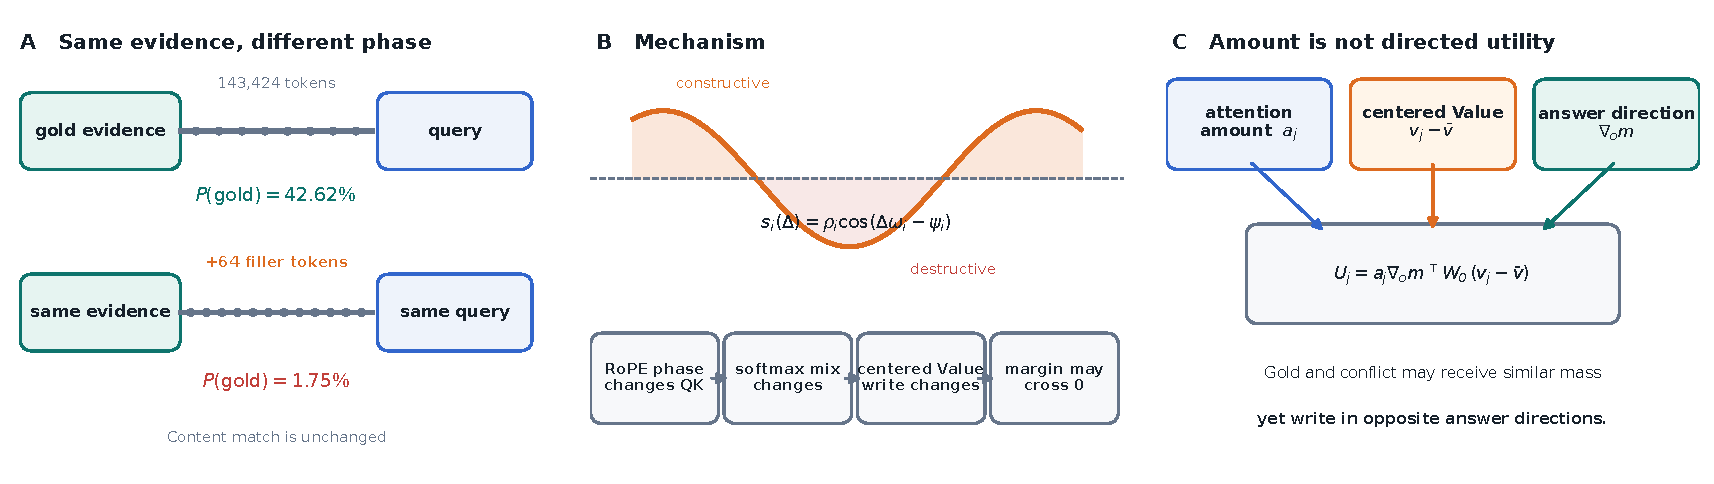
\includegraphics[width=0.98\textwidth]{figures/overview.pdf}
  \caption{Our problem--analysis--repair loop.  Changing the separation
  between fixed evidence and a query changes RoPE phase before softmax.  An
  unfavorable phase suppresses the gold QK score, competing tokens take more
  probability mass, and the altered Value write causes later representations
  to diverge.  \method repairs the same bottleneck: local tokens retain
  standard RoPE, while remote candidates receive a position-free semantic
  proposal and are then consumed by the original post-RoPE attention.}
  \label{fig:overview}
\end{figure*}

\textbf{We locate a phase-sensitive bottleneck before the softmax.}
RoPE rotates each two-dimensional query/key pair at a different frequency.
For fixed pre-RoPE content vectors, the contribution of pair $i$ at relative
distance $\Delta$ is
\begin{equation}
  s_i(\Delta)
  = A_i\cos(\Delta\omega_i)+B_i\sin(\Delta\omega_i).
  \label{eq:intro-phase}
\end{equation}
Thus RoPE couples semantic compatibility to a distance-dependent phase.  The
aggregate score need not decrease monotonically, but a relevant key can be
suppressed whenever high-energy frequency pairs interfere destructively.  On
Qwen3-8B, summing the 64 analytically reconstructed pair contributions matches
the measured first-layer score across four evidence--query distances with at
most $1.98\times10^{-3}$ absolute error.  This isolates phase: the pre-RoPE
queries and keys are exactly unchanged in that experiment.

\textbf{The initial score change becomes a representation change.}
Softmax turns a relative score change into an exponential attention-ratio
change.  The changed attention weights alter the Value written into the query
residual; subsequent layers therefore do not repeatedly rotate the same
query.  They project new pre-RoPE queries and keys from already divergent
hidden states.  We record the complete attention, MLP, and residual vectors in
a 36-layer Qwen3-8B transition and exactly replay every BF16 residual update.
Although the query embedding difference is zero, the first attention branch
creates a nonzero residual difference; its norm reaches 312.68 by the final
layer.  Causally patching the successful residual state into the failed run at
layer 16 changes the output margin from $-2.75$ to $+0.625$, and patching at
layer 20 restores it to $+1.00$.

\textbf{The diagnosis directly specifies the repair.}
Local order remains important for syntax and within-evidence structure, so
removing RoPE globally is unnecessarily disruptive.  Conversely, fine-grained
distance should not by itself eliminate a remote token whose content is
strongly compatible with the query.  We therefore introduce \method
(Semantic-Augmented Global Evidence retrieval for RoPE models).  Its
conservative \methodpost variant keeps sink and recent tokens, proposes remote
tokens with pre-RoPE QK, and spends the remaining 2\% budget on those
candidates.  It then retrieves the original K/V and applies the model's exact
post-RoPE score, softmax, and Value aggregation.  The intervention changes
which remote tokens may compete, but not how selected tokens are scored or
consumed.

\textbf{Controlled held-out evaluation supports the mechanism-derived design.}
On a frozen set of 24 unseen two-hop instances at each of 8K, 16K, 32K, and
64K, \methodpost reduces aggregate geometric \GoldPPL from 10.851 under full
attention to 4.859 and raises first-token accuracy from 33.3\% to 47.9\%.
Against exact post-RoPE Top-2\% selection at the same budget, it lowers mean
NLL by 0.643 at 16K and 0.691 at 32K, corresponding to $1.90\times$ and
$2.00\times$ gold-token likelihood ratios; both 95\% confidence intervals
exclude zero.  The 64K interval narrowly crosses zero, and current experiments
are synthetic and use a full pre-RoPE scan.
Accordingly, we claim a controlled mechanism and repair---not universal
generalization or an end-to-end speedup.

The paper makes three contributions.  First, it formalizes
\emph{phase-sensitive retrieval failure}: a fixed semantic match can receive
different attention priority solely through RoPE-relative phase.  Second, it
connects this first-layer effect to attention mass, residual divergence, and
the output decision using exact finite-difference replay and activation
patching.  Third, it derives a local-position/global-semantics attention rule
from the diagnosis and demonstrates its value under held-out, matched-budget
evaluation.
